\documentclass[12pt]{article}
\usepackage{fancyhdr}
\usepackage{color}
\usepackage{multicol}
\usepackage{fancyvrb}
\usepackage{enumitem}
\usepackage{graphicx}
\usepackage{sectsty}
\usepackage{amsmath}
\usepackage{amssymb}
\usepackage{hyperref}
\usepackage{array}
\newcommand{\sectionbreak}{\clearpage}

\usepackage{tikz}
\usepackage{tkz-euclide}
\usetkzobj{all}

\allsectionsfont{\centering}

\usepackage{draftwatermark}
	\SetWatermarkText{\copyright wolf-math.com}
	\SetWatermarkScale{4}
	\SetWatermarkLightness{1}

\usepackage[margin=1in, headsep=0pt]{geometry}
\setlength{\parindent}{0cm}
\pagestyle{empty}

\begin{document}

Mr. Wolf \\ www.wolf-math.com

\section*{Linear Relations}

\subsection*{Goals}

\textbf{SWBAT} determine the differences between linear relationships and non-linear relationships.\\

\textbf{SWBAT} determine the slope of a line by using the slope formula and by using a graph.\\

\textbf{SWBAT} graph linear functions by using slope intercept form.\\

\textbf{SWBAT} create an equation given either 2 points, or a point and slope.\\

\textbf{SWBAT} convert from point-slope form to slope-intercept form.



\subsection*{Standards} 

\textbf{Reasoning with Equations and Inequalities \hfill	A-REI}\\

 Solve equations and inequalities in one variable\\
 
3.	 Solve linear equations and inequalities in one variable, including
equations with coefficients represented by letters.\\



\subsection*{Connections}

\textbf{Now} we are learning how to create, graph, and solve linear equations.\\

\textbf{Later} we will learn what happens when two linear equations are multiplied, and it turns into a quadratic.


\pagebreak


\section*{Linear Functions}

\textbf{What is a Linear Function?} \\

\vspace{1in}

\textbf{How do we know something is a linear function?}\\



\begin{enumerate}
\item there is 1 $x$ without an exponent

\item this $x$ is not in the denominator of a fraction

\item there is only 1 variable \\

\end{enumerate}
\begin{center}

\begin{tabular}{ l | c }
  \textbf{Linear equations} & \textbf{Nonlinear equations}  \\ \hline
  $4x-5y=16$ & $2x+6y^2=-25$  \\
  $x=10$ & $y=\sqrt{x}+2$  \\
  $y=\frac{1}{2}x$ & $y=\frac{1}{x}$\\
\end{tabular}
\end{center}

\begin{Large}
\textbf{You Try}
\end{Large}

\textbf{State Whether each Function is a Linear Function} \textit{and why}

\begin{enumerate}
\item $f(x)=8-\frac{3}{4}x$\\

\vspace{1in}

\item $g(x)=\frac{2}{x}$\\

\vspace{1in}

\item $h(x)=3x-4$\\
\end{enumerate}

\pagebreak


\section*{Slope}

\textbf{What is Slope?} -- (Not the definition you see below)
\vspace{1in}



\textbf{Definition}\\
$$Slope=\frac{\text{change\, in\,}y}{\text{change\, in\,} x}$$
\indent What does "change in" mean?\\

\vspace{1in}

If we have 2 points we can find the slope between them\\

\begin{multicols}{2}
\begin{enumerate}
\item $(3,2),(8,12)$ \\

\item $(-1,4),(3,-8)$\\

\item $(-2,-5),(-7,10)$\\

\item $(4,4), (10,12)$\\
\end{enumerate}
\end{multicols}

\begin{Large}
\textbf{You Try}
\end{Large}

\begin{enumerate}
\item Determine the rate of change of the graph\\ 

%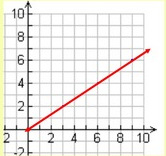
\includegraphics[scale=.5]{rateofchange.jpg}\\

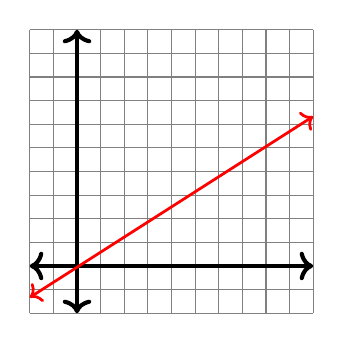
\begin{tikzpicture}[scale=.3]

   \tkzInit[xmax=10,ymax=10,xmin=-2,ymin=-2]
   \tkzGrid
 %  \tkzAxeXY

\draw[line width=1.5pt,<->](0,10)--(0,-2);
\draw[line width=1.5pt,<->](-2,0)--(10,0);
\draw[red,line width=1pt,<->](-2,-1.3333)--(10,6.33333);


\end{tikzpicture}

\item $(8,-3),(6,-2)$\\

\item $(-2,-5),(8,-15)$\\
\end{enumerate}

\pagebreak

\section*{Types of Slope}

\textbf{There are $4$ types of slope.}

\begin{enumerate}
\begin{multicols}{2}
	\item Positive\\ 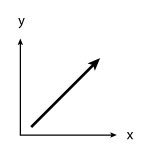
\includegraphics[scale=.6]{positive.jpg}\\
	
	\item Negative\\ 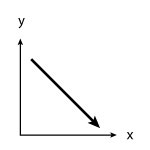
\includegraphics[scale=.6]{negative.jpg}\\
	
	\item Zero\\ 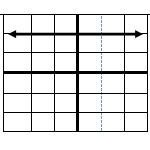
\includegraphics[scale=.6]{0.jpg}\\
	
	\item undefined\\ 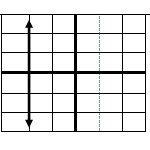
\includegraphics[scale=.6]{undefined.jpg}\\
\end{multicols}
\end{enumerate}

We can see how this works out in the equation of a graph.\\

\begin{enumerate}
\item $y=3x+6$\\

\item $y=-\frac{4}{3}x+2$\\

\item $x=10$\\

\item $y=10$\\
\end{enumerate}

\pagebreak

\section*{Graphs of Linear Functions}

\textbf{$y=mx+b$} is called \textit{slope-intercept form}. This is the form that is most commonly used for graphing linear equations, although we'll see at least one other later on. \\

We can use a t-chart to graph the equation. $y=3x-7$\\ 

\begin{center}

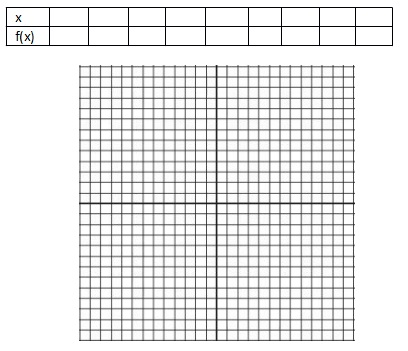
\includegraphics[scale=.9]{graphchart.jpg}

\end{center}

The y-intercept is the $b$ value. We just take this and graph it on the vertical axis. The slope is the $m$ value. To graph we begin by finding the intercept, then graph the rest by using the slope.\\

Graph $y=-\frac{1}{2}x+1$

\begin{center}
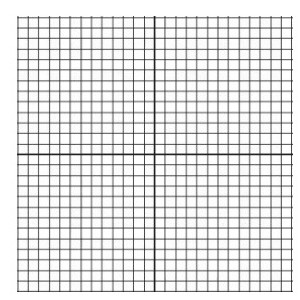
\includegraphics[scale=1]{graph.jpg}
\end{center}


\pagebreak

\section*{Point-Slope Form}

How to find the equation of a line that passes through two different points.\\

This is a job for \textit{Point-Slope Form}!\\

\begin{Large}
$$y-y_1=m(x-x_1)$$\\
\end{Large}

All that is needed is 2 points, or 1 point and a slope. Either way the slope is going to be discovered. $y_1$, and $x_1$ are from the point $(x_1,y_1)$. \\

If I need a line to pass through the point $(3,5)$ and has slope of $4$, then I just need to plug my pieces into the form.\\

$x_1=3$\\
$y_1=5$\\
$m=4$\\

so my equation looks like...\\

$$y-5=4(x-3)$$ 

That's it!\\

\textbf{You Try:} Write an equation that goes through the indicated point, with the indicated slope, then graph.

\begin{multicols}{2}

$(-1,3)$ slope$=\frac{1}{2}$\\

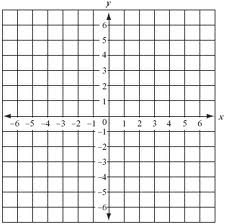
\includegraphics[scale=.9]{graphing.jpg}

$(3,-4)$ slope$=\frac{4}{3}$\\

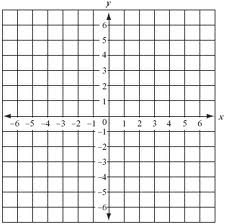
\includegraphics[scale=.9]{graphing.jpg}

\end{multicols}

\pagebreak


\subsection*{With 2 Points}

The process is exactly the same with 2 points, except that the slope needs to be calculated. \\



\textbf{Step 1:} Calculate the slope $\frac{y_1-y_2}{x_1-x_2}$\\

\textbf{Step 2:} Pick which point you like better.\\

\textbf{Step 3:} Use slope from step 1, your favorite point, then plug  in to point-slope form.\\

\hrulefill


Find the equation of the line passing through the points $(1,1)$, and $(-3,5)$\\

\textbf{Step 1:} $\frac{1- -3}{1-5}=\frac{2}{-4}=-\frac{1}{2}$\\

\textbf{Step 2:} I think $(1,1)$ is a fine looking point, so I'm going to use it!\\

\textbf{Step 3:} $(y-1)=\frac{1}{2}(x-1)$\\

\hrulefill

\textbf{You Try:} Write the equation of the line passing through the points, the graph. 


\begin{enumerate}
\begin{multicols}{2}

\item $(2,3)$ and $(4,4)$\\
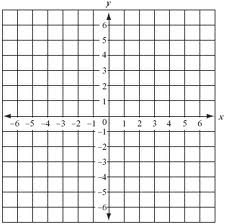
\includegraphics[scale=.7]{graphing.jpg}

\item $(-1,-5)$ and $(1,-3)$\\
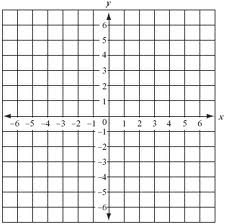
\includegraphics[scale=.7]{graphing.jpg}

\item $(-12,-20)$ and $(-30,-40)$\\
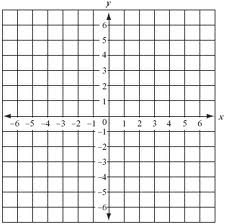
\includegraphics[scale=.7]{graphing.jpg}

\item $(-14,-5)$ and $(-8,3)$\\
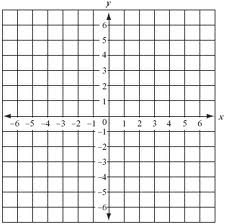
\includegraphics[scale=.7]{graphing.jpg}
\end{multicols}
\end{enumerate}


\pagebreak

\section*{Converting Forms}

\noindent $ax+by=c$ is called standard form.\\ 

\noindent Convert  $2y+3x=6$ to slope-intercept form. Do it by solving for $y$.\\

$2y=6-3x$\\

$y=\frac{6-3x}{2}$\\

$y=3-\frac{3}{2}x$\\

$y=-\frac{3}{2}x+3$\\

\noindent \textbf{You Try} Convert $4y+3x=12$ to slope-intercept form.\\

\vspace{23mm}

\noindent \textbf{Converting to slope-intercept form.} \\

\noindent Convert $y-7=\frac{3}{4}(x+20)$ to slope-intercept form\\

$y-7=\frac{3}{4}x+15$ \textbf{**distribute the $\frac{3}{4}$**}\\

$y=\frac{3}{4}x+22$\\

\begin{enumerate}
\item $(y-1)=\frac{1}{2}(x-4)$\\

\item $(y-3)=\frac{10}{9}(x-9)$\\

\item $(y+1)=4(x+1)$\\

\item $(y-8)=\frac{5}{9}(x-18)$\\

\end{enumerate}

\pagebreak


\section*{Review of Linear Equations}


\textbf{Identify the function as linear} or nah -- Circle the linear equations

\begin{enumerate}
\begin{multicols}{2}

\item $y=2x-1$ \\

\item $3x+6y=4$\\

\item $y=x^2$\\

\item $y=\frac{1}{x}$\\

\item 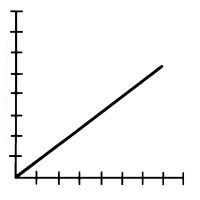
\includegraphics[scale=.5]{linear.jpg}

\item $xy=13$\\

\item $\frac{x}{y}=10$\\

\item $\frac{y}{x}=10$\\

\item $3x-y=10$\\

\item 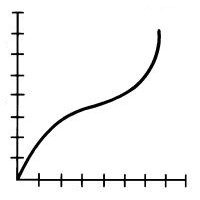
\includegraphics[scale=.5]{nonlinear.jpg}

\end{multicols}
\end{enumerate}

\hrulefill

\textbf{Calculate the slope $\frac{y_1-y_2}{x_1-x_2}$}

\begin{enumerate}[resume]
\begin{multicols}{2}

\item $(-2,7),(8,13)$\\

\item $(0,0),(0,10)$\\

\item $(-6,-2),(-3,-4)$\\

\item $(5,2),(9,2)$\\

\end{multicols}
\end{enumerate}

\hrulefill

\textbf{Graph the lines}

\begin{enumerate}[resume]
\begin{multicols}{2}

\item $y=\frac{3}{2}x-4$\\

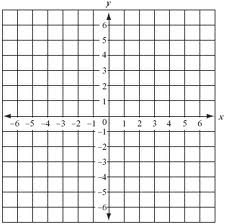
\includegraphics[scale=.7]{graphing.jpg}

\item $y=\frac{-1}{5}x+3$\\

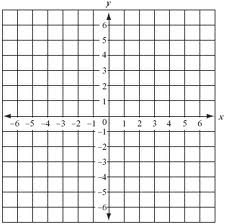
\includegraphics[scale=.7]{graphing.jpg}

\end{multicols}
\end{enumerate}

\pagebreak

\textbf{Write an equation in Point-Slope Form} $y-y_1=m(x-x_1)$\\

\begin{enumerate}[resume]
\begin{multicols}{2}

\item $(2,3) m=9$\\

\item $(-1,-6) m=\frac{4}{5}$\\

\item $(-3,-9), (2, 1)$\\

\item $(7,0),(9,2)$\\

\end{multicols}
\end{enumerate}

\hrulefill

\textbf{Convert from Point-Slope to Slope-Intercept Form}\\

\begin{enumerate}[resume]
\begin{multicols}{2}

\item $y-3=\frac{1}{2}(x-6)$\\

\item $y+16=\frac{8}{3}(x-3)$\\

\item $y-10=\frac{3}{4}(x+20)$\\

\item $y+212=\frac{9}{5}(x-100)$\\


\end{multicols}
\end{enumerate}

\hrulefill

\textbf{Pre-assessment:}  This section for extra credit on quiz\\

Solve for $x$ and $y$. Use substitution, elimination, or graphing.\\

$$2x-3y=-2$$

$$4x+y=24$$\\


\pagebreak

\hfill NAME:\underline{\hspace{3in}}\\

\section*{Linear Equations Test}

\textbf{Identify the function as linear} or not -- Circle the linear equations

\begin{enumerate}
\begin{multicols}{2}

\item $xy=12$ \\

\item $\frac{x}{y}=11$\\

\item $3x-y=9$\\

\item 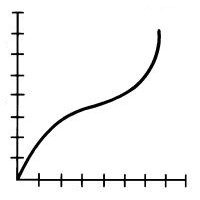
\includegraphics[scale=.5]{nonlinear.jpg}

\item $y=2x-3$\\

\item $x+6y=5$\\

\item $y=x^3$\\

\item 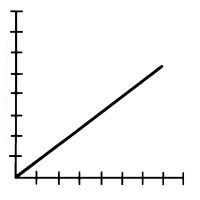
\includegraphics[scale=.5]{linear.jpg}

\end{multicols}
\end{enumerate}

\hrulefill

\textbf{Calculate the slope $\frac{y_1-y_2}{x_1-x_2}$}

\begin{enumerate}[resume]
\begin{multicols}{2}

\item $(-3,5),(7,12)$\\

\item $(-1,-1),(-1,9)$\\

\item $(-5,-1),(-2,-3)$\\

\item $(6,3),(10,3)$\\

\end{multicols}
\end{enumerate}

\hrulefill

\textbf{Graph the lines}

\begin{enumerate}[resume]
\begin{multicols}{2}

\item $y=\frac{3}{2}x-4$\\

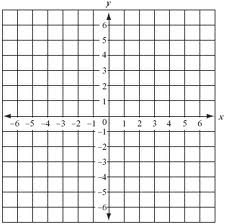
\includegraphics[scale=.7]{graphing.jpg}

\item $y=\frac{-2}{5}x+5$\\

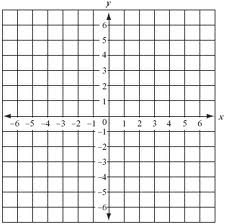
\includegraphics[scale=.7]{graphing.jpg}

\end{multicols}
\end{enumerate}

\pagebreak

\textbf{Write an equation in Point-Slope Form} $y-y_1=m(x-x_1)$\\

\begin{enumerate}[resume]
\begin{multicols}{2}

\item $(7,3) m=3$\\

\item $(-2,-4) m=\frac{6}{11}$\\

\item $(-4,-9), (1, 1)$\\

\item $(-8,3),(-3,8)$\\

\end{multicols}
\end{enumerate}

\hrulefill

\textbf{Convert from Point-Slope to Slope-Intercept Form}\\

\begin{enumerate}[resume]
\begin{multicols}{2}

\item $y-5=\frac{1}{2}(x-5)$\\

\item $y+10=\frac{9}{5}(x-5)$\\

\item $y-12=\frac{4}{3}(x+15)$\\

\item $y-20=\frac{5}{8}(x-32)$\\


\end{multicols}
\end{enumerate}

\hrulefill

\textbf{Extra Credit:} Freezing is at $32^{\circ}F$, which is also $0^{\circ}C$. Boiling is at $212^{\circ}F$ or $100^{\circ}C$. Using this information, write a linear equation that converts between the two units of temperature.

\end{document}